\subsection{Pretrained VidLMs:}
Models used in this benchmark of VILMA.
\textbf{Unimodel Models:}
Modelos basados en solo texto (i.e. text-only MLs), tenemos 2 tipos:

decoder-only models: estos se enfocan en generar y predecir aspectos de tareas del lenguage como modelado del lenguaje, completacion de texto y generacion de texto, para los benchamarks se tiene:
\begin{itemize}
\item GPT2-2
\end{itemize}
Encoder-decoder models:Estos son los mismos que sequence-to-sequence, estos modelos procesan como input una sequencia a la cual se le debe asignar otra sequencia como respuesta, como por ejemplo traducion, resumir un texto y responder preguntas, para los benchmark se tiene:
\begin{itemize}
\item T5
\item BART
\item BOTH
\end{itemize}
and for both:
\begin{itemize}
\item OPT
\end{itemize}
Al igual que VALSE se calcula los perplexity values para ambos caption y foil, y tomamos el text intput con menor perpelxiti escore.
Parametros usados:
\begin{itemize}
\item GPT-2 124M
\item OPT 6.7B
\end{itemize}


\textbf{Image Language Models:}
La definicion de una Image Language model se encuentra en la subsecion \ref{ilm}.
Los modelos usados para los benchmarks son:
\begin{itemize}
\item CLIP
\item BLIP
\end{itemize}
Ambos con OPT model.
 
\textbf{Video Language Models:}
La definicion de Video Lnaguage Model se encuentra subsection \ref{vlm}.
Listado de Modelos usados pata benchmark:
\begin{itemize}
\item ClipBERT:
\begin{itemize}
\item Text-encoder: BERT
\item Video-encoder: Resnet-50
\item Features:
\begin{enumerate}
\item Este pretrainet usa solamente imagenes.
\item No aprende orden temporal: El escore de similitud de Video-text es el promedio de el escore de similitud de frame-text.
\end{enumerate}
\end{itemize}
\end{itemize}

\begin{itemize}
\item UniVL:
\begin{itemize}
\item Text-encoder: BERT
\item Video-encoder: S3D
\item Features:
\begin{enumerate}
\item Dual-stream Architecture: UniVL employs a dual-stream architecture consisting of a video encoder and a text encoder. The video encoder processes the visual information, while the text encoder processes the language information. Both encoders are built using Transformer layers.
\item Cross-modal Transformer: After encoding the video and text separately, UniVL employs a cross-modal Transformer to fuse the information from both modalities. This cross-modal Transformer is crucial for understanding and generating coherent video-language representations.
\item UniVL is pretrained on HowTo100M.
\end{enumerate}
\end{itemize}
\end{itemize}

\begin{itemize}
\item VideoCLIP:
\begin{itemize}
\item Text-encoder: BERT
\item Video-encoder: S3D
\item Features:
\begin{enumerate}
\item it uses mean pooling to fuse modalities, this is similar to the Video-text similarity score for ClipBERT.
\item VideoCLIP is pretrained on HowTo100M.
\end{enumerate}
\end{itemize}
\end{itemize}

\begin{itemize}
\item FiT:
\begin{itemize}
\item Text-encoder: BERT
\item Video-encoder: TimeSFormer
\item Features:
\begin{enumerate}
\item it be able to be pretrained on images(CC3M) and videos(W2).
\item it creates a shared video-text space through contrastive learning. 
\end{enumerate}
\end{itemize}
\end{itemize}

\begin{itemize}
\item CLIP4Clip:
\begin{itemize}
\item Text-encoder: BERT
\item Video-encoder: Resnet-50
\item Features:
\begin{enumerate}
\item Its primary goal is to enable effective retrieval of videos based on textual descriptions and vice versa. 
\item Video Representation: It uses the Clip video encoder, processing each frame as if it were an image.
\item Text Representation: It use the Clip text encoder. Textual queries or descriptions are encoded into embeddings that reside in the same space as the video frame embeddings.
\item Strategy for modeling space-time:
\begin{itemize}
\item Simple aggregation methods like mean pooling over frame embeddings.
\item Sophisticated techniques such as attention mechanisms to capture the temporal dependencies between frames.
\end{itemize}
\end{enumerate}
\end{itemize}
\end{itemize}

\begin{itemize}
\item 	VIOLET:
\begin{itemize}
\item Text-encoder: BERT
\item Video-encoder: Video Swin Transformer
\item Features:
\begin{enumerate}
\item it be able to be pretrained on images(CC3M) and videos(YT-Temporal, WebVid).
\item Spatial and temporal dimensions of the video inputs are modelled by positional embeddings considering both spatial and temporal ordering. 
\end{enumerate}
\end{itemize}
\end{itemize}

\begin{itemize}
\item 	X-Clip:
\begin{itemize}
\item Text-encoder: BERT
\item Video-encoder: Resnet-50, or ViT
\item Features:
\begin{enumerate}
\item Contrastive Loss: During training, the model uses a contrastive loss function, typically a variant of the InfoNCE (Information Noise Contrastive Estimation) loss. This loss encourages the similarity scores of matching video-text pairs to be higher than those of non-matching pairs.
\item It introduces the Attention Over Similarity Matrix (AOSM) module, enabling it to focus on essential frames and words while reducing the impact of irrelevant ones during retrieval.
\end{enumerate}
\end{itemize}
\end{itemize}

MCQ(Definition in section\ref{mcq_model}): A pretext task using Multiple Choice Questions (MCQ) was introduced for video-text pretraining, utilizing a dual-encoder approach. This involved a parametric module named BridgeFormer, which links local features from both VideoFormer and TextFormer to address multiple-choice questions through a contrastive learning objective. This method enhances the semantic connections between video and text representations, improving detailed semantic associations between the two modalities. Furthermore, it ensures high efficiency for retrieval, and the BridgeFormer can be omitted for downstream tasks.

\begin{itemize}
\item Singularity:
\begin{itemize}
\item Text-encoder: BERT
\item Video-encoder: ViT
\item Features:
\begin{enumerate}
\item In the training phase, a single frame is randomly selected as input, and a video-level prediction is made using the information from this frame and its corresponding text input. During inference, multiple frames are uniformly sampled, and their encoded image-level representations are combined early on as input to the multi-modal encoder, see Figure \ref{fig:singularity_m}.
\end{enumerate}
\end{itemize}
\end{itemize}

\begin{figure}[h]
    \centering
    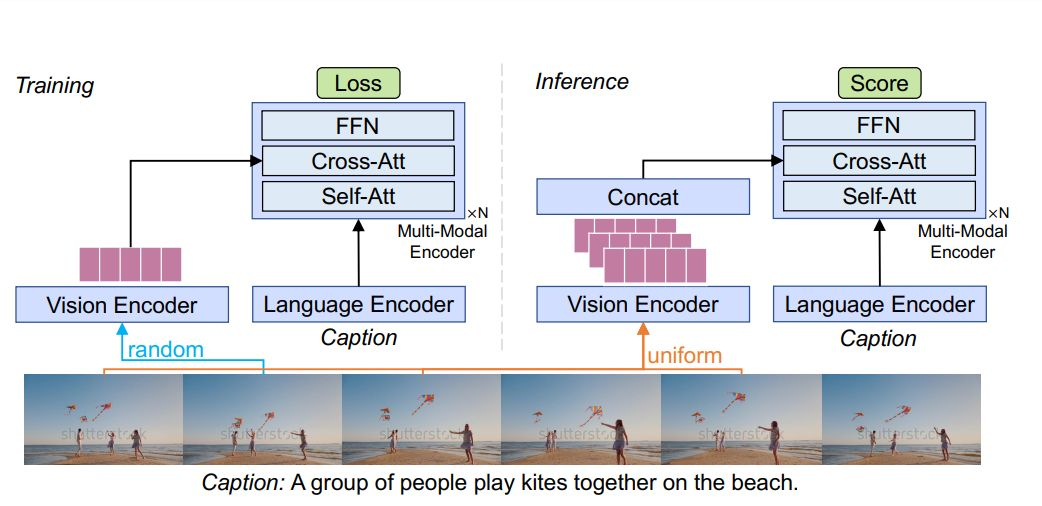
\includegraphics[width=0.55\textwidth]{singularity_model}
    \caption{Process of the Singularity model}
    \label{fig:singularity_m}
\end{figure}

UniPerceiver: It is used for perception tasks in videos. The model is designed to handle zero-shot and few-shot learning situations. UniPerceiver was inspired by the Transformer architecture but uses CNN for a variety of modalities such as text, images and videos. See Figure \ref{fig:uniPerceiver_m}

\begin{figure}[h]
    \centering
    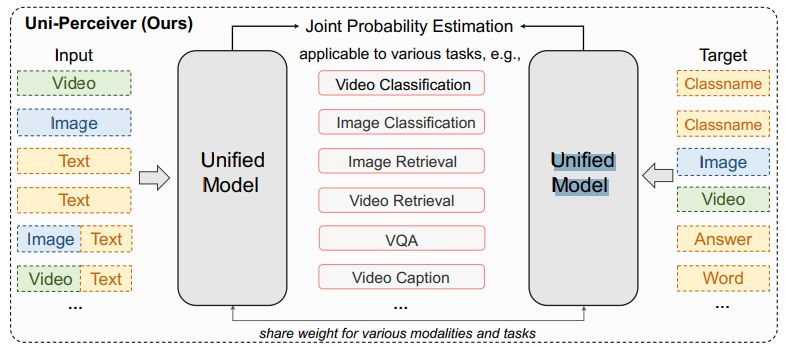
\includegraphics[width=0.55\textwidth]{uniPerceiver_model}
    \caption{Process of the UniPerceiver model}
    \label{fig:uniPerceiver_m}
\end{figure}

Merlot Reserve: It has a better understanding of temporal space for videos by combining audio, subtitles, and video frames. The model learns by substituting bits of text and audio with a MASK token and selecting the one that fits best describes the image. 

\begin{itemize}
\item VindLU:
\begin{itemize}
\item Text-encoder: BERT
\item Video-encoder: BEiT (BERT Pre-Training of image transformer)
\item Features:
\begin{enumerate}
\item Use a visual-text contrastive objective.
\item These models add the following steps to improve their result: the inclusion of temporal attention, integration of a multimodal fusion encoder, adoption of masked modeling pretraining objectives, joint training on images and videos, utilization of additional frames both in fine-tuning and inference stages, model-parameter and data scaling.
\end{enumerate}
\end{itemize}
\end{itemize}